\documentclass{beamer}

\usepackage[utf8]{inputenc}
\usetheme{default}

\usepackage{listings}
\lstset{
basicstyle=\small\ttfamily,
columns=flexible,
breaklines=true
}

\usepackage{epstopdf}
\usepackage{multicol}
\usepackage{caption}

\makeatletter
\DeclareMathSizes{\f@size}{10}{7}{7}
\makeatother

\title[66.20/86.37]{U.B.A. - Facultad de Ingeniería\\\vspace{0.25cm} 66.20/86.37 Organización de Computadoras
\\Arquitecturas}
\author{Práctica}
\date{2$^{do}$ cuatrimestre 2020}


\begin{document}
\begin{frame}
\titlepage % Print the title page as the first frame
\end{frame}

\begin{frame}
\frametitle{Clasificación de ISAs}
\begin{center}
 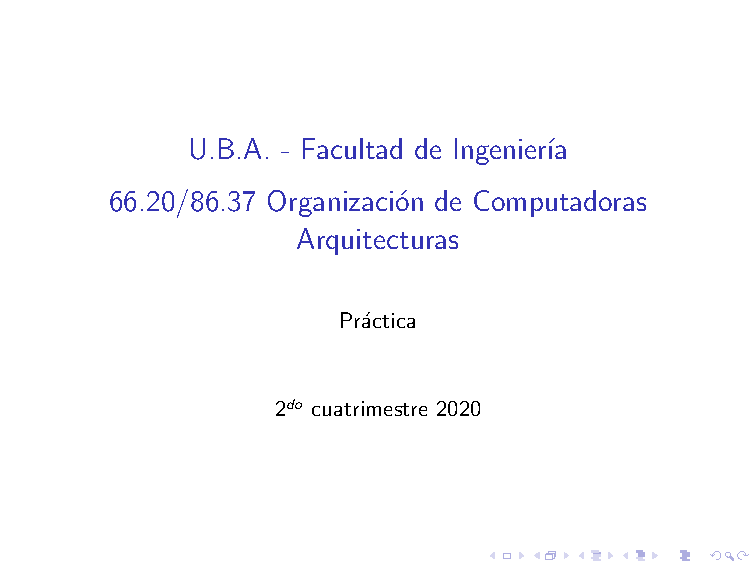
\includegraphics[scale=.45,keepaspectratio=true]{ISA.png}
\end{center}
\end{frame}

\begin{frame}
 \frametitle{Clasificación de ISAs}
 \begin{itemize}
  \item Modelo de pila: 
Los operandos están implícitamente en el tope del stack y el hardware debe evaluar la expresión en un solo orden y cargar un operando múltiples veces.
\item Modelo de acumulador: 
En una arquitectura de acumulador un operando está implícito en el acumulador.
\item Modelo de registros de propósito general: 
Aquí se tienen únicamente operandos explícitos, ya sea que estén ubicados en registros o en memoria.
\item Modelo de carga y almacenamiento: 
En este tipo de arquitectura, la memoria solo puede ser accedida a través de instrucciones de carga y almacenamiento (load/store). 
 \end{itemize}
\end{frame}


\begin{frame}
 \frametitle{Tipo de instrucciones en MIPS}
 \begin{itemize}
  \item Load / Store: únicas que acceden a memoria.
  \item Computational: realizadas en la ALU.
  \item Jump / Branch: saltos incondicionales y condicionales.
  \item Miscelaneas: Serialización de instrucciones, Excepciones (syscall), Moves condicionales, Prefetch, NOPs.
  \item Coprocessors y FPU.
 \end{itemize}
\end{frame}



\begin{frame}
 \frametitle{Endianess}
Todo el conjunto de instrucciones es direccionado por bytes y se provee acceso por bytes (8 bits), mitad de palabra (half words) (16 bits), por palabra (words) (32 bits).

\bigskip

Hay dos convenciones para ordenar los bytes en un objeto. \textbf{Little Endian} y \textbf{Big Endian}.
 \end{frame}
 
\begin{frame}
 \frametitle{Endianess}

El orden \textbf{Little Endian} coloca el byte cuya dirección "x . . . x000” en la posición menos significativa. Los bytes entonces son numerados:

  \begin{center}
 \includegraphics[scale=.7,keepaspectratio=true]{little_endian.png}
\end{center}


El orden \textbf{Big Endian} coloca el byte cuya dirección es “x . . . x000”  en la posición más significativa. Los bytes entonces son numerados:

\begin{center}
 \includegraphics[scale=.7,keepaspectratio=true]{big_endian.png}
\end{center}

 \end{frame}


\begin{frame}
 \frametitle{Alineación}
 En varias computadoras, los accesos a objetos más grandes que un byte deben estar alineados.
 \begin{itemize}
  \item Un objeto de tamaño s bytes en la dirección de bytes A está alineado si
    A mod s = 0.
  \item Esto se fuerza en muchas arquitecturas porque el hardware accede a
    memoria típicamente alineado a múltiplos de word o double-word.
 \end{itemize}
\bigskip
 ¿Qué puede ocurrir a nivel de accesos a memoria si se accede a datos no alineados y la arquitectura lo permite?
    
\end{frame}

\begin{frame}
 \frametitle{Modos de direccionamiento}
Se presentan varios modos de direccionamiento: 
\begin{multicols}{2}
\begin{itemize}
 \item Register
 \item Immediate
 \item Displacement
 \item Register indirect
 \item Indexed
 \item Direct or Absolute
 \item Memory indirect
 \item Autoincrement
 \item Autodecrement
 \item Scaled
 \end{itemize}
\end{multicols}

MIPS implementa 2 modos de direccionamiento: Immediate y Displacement, ambos con immediate de 16 bits.
    
Usando el registro 0 se consigue Absolute, y con displacement 0 se consigue Register indirect.
\end{frame}

\begin{frame}[fragile]
\frametitle{Modos de direccionamiento}

\begin{lstlisting}
    Immediate:		add	$t1, $t2, 10	
    Displacement:	lw	$t1, 30($t2)
    Absolute:		sb	$t1, 40($0)
    Indirect:		sw	$t1, 0($t2)
\end{lstlisting}
\end{frame}


\begin{frame}
 \frametitle{Encoding MIPS} 
 Hay 3 formatos de encoding posibles en MIPS
 \begin{itemize}
  \item I-type (Immediate)
  \item R-type (Register)
  \item J-type (Jump)
 \end{itemize}
\end{frame}

\begin{frame}
 \frametitle{Encoding MIPS} 
 
 \begin{center}
 \includegraphics[scale=.4,keepaspectratio=true]{tipos_instruccion.png}
\end{center}
 \end{frame}


\begin{frame}
 \frametitle{Encoding MIPS} 

 Viendo el detalle de las instrucciones J-type vemos que hay un offset de 26 bits left-shifted 2 bits, para formar los 28 lsb de la direccion destino del salto (las regiones de salto están alineadas a 256MB, y la región está determinada por los 4 msb de PC).
 
 \bigskip

 ¿Por qué se puede (y conviene) tomar los 26 bits como desplazados a la izquierda 2 bits?
\end{frame}

     
\end{document}
